%TC第29.1节练习 4、5
%TC第29.2节练习 2、4、6
%TC第29.3节练习 5
%TC第29.4节练习 2
%%%%%%%%%%%%%%%%%%%%%%%%%%%%%%%%%%%%%%%%%%%%%%%%%%%%%%%%%%%%%%%%
% \documentclass[11pt, a4paper, UTF8]{ctexart}
% %%%%%%%%%%%%%%%%%%%%%%%%%%%%%%%%%%%
% File: preamble.tex
%%%%%%%%%%%%%%%%%%%%%%%%%%%%%%%%%%%

\usepackage[top = 1.5cm]{geometry}

% Set fonts commands
\newcommand{\song}{\CJKfamily{song}} 
\newcommand{\hei}{\CJKfamily{hei}} 
\newcommand{\kai}{\CJKfamily{kai}} 
\newcommand{\fs}{\CJKfamily{fs}}

\newcommand{\me}[2]{\author{{\bfseries 姓名:}\underline{#1}\hspace{2em}{\bfseries 学号:}\underline{#2}}}

% Always keep this.
\newcommand{\noplagiarism}{
  \begin{center}
    \fbox{\begin{tabular}{@{}c@{}}
      请独立完成作业,不得抄袭。\\
      若得到他人帮助, 请致谢。\\
      若参考了其它资料,请给出引用。\\
      鼓励讨论,但需独立书写解题过程。
    \end{tabular}}
  \end{center}
}

% Each hw consists of three parts:
% (1) this homework
\newcommand{\beginthishw}{\part{作业}}
% (2) corrections (Optional)
\newcommand{\begincorrection}{\part{订正}}
% (3) any feedback (Optional)
\newcommand{\beginfb}{\part{反馈}}

% For math
\usepackage{amsmath}
\usepackage{amsfonts}
\usepackage{amssymb}

% Define theorem-like environments
\usepackage[amsmath, thmmarks]{ntheorem}

\theoremstyle{break}
\theorembodyfont{\song}
\theoremseparator{}
\newtheorem*{problem}{题目}


\theoremheaderfont{\kai\bfseries}
\theoremseparator{:}
% \newtheorem*{remark}{注}
\theorempostwork{\bigskip\hrule}
\newtheorem*{solution}{解答}
\theorempostwork{\bigskip\hrule}
\newtheorem*{revision}{订正}

\theoremstyle{plain}
\newtheorem*{cause}{错因分析}
\newtheorem*{remark}{注}

\theoremstyle{break}
\theorempostwork{\bigskip\hrule}
\theoremsymbol{\ensuremath{\Box}}
\newtheorem*{proof}{证明}

\renewcommand\figurename{图}
\renewcommand\tablename{表}

% For figures
% for fig with caption: #1: width/size; #2: fig file; #3: fig caption
\newcommand{\fig}[3]{
  \begin{figure}[htp]
    \centering
      \includegraphics[#1]{#2}
      \caption{#3}
  \end{figure}
}

% for fig without caption: #1: width/size; #2: fig file
\newcommand{\fignocaption}[2]{
  \begin{figure}[htp]
    \centering
    \includegraphics[#1]{#2}
  \end{figure}
}
% \usepackage{float}
% \usepackage{amsmath}
% \usepackage{graphicx}
% \usepackage{listings}
% \usepackage{xcolor}
% \usepackage{enumerate}
\documentclass[11pt, a4paper, UTF8]{ctexart}
%%%%%%%%%%%%%%%%%%%%%%%%%%%%%%%%%%%
% File: preamble.tex
%%%%%%%%%%%%%%%%%%%%%%%%%%%%%%%%%%%

\usepackage[top = 1.5cm]{geometry}

% Set fonts commands
\newcommand{\song}{\CJKfamily{song}} 
\newcommand{\hei}{\CJKfamily{hei}} 
\newcommand{\kai}{\CJKfamily{kai}} 
\newcommand{\fs}{\CJKfamily{fs}}

\newcommand{\me}[2]{\author{{\bfseries 姓名:}\underline{#1}\hspace{2em}{\bfseries 学号:}\underline{#2}}}

% Always keep this.
\newcommand{\noplagiarism}{
  \begin{center}
    \fbox{\begin{tabular}{@{}c@{}}
      请独立完成作业,不得抄袭。\\
      若得到他人帮助, 请致谢。\\
      若参考了其它资料,请给出引用。\\
      鼓励讨论,但需独立书写解题过程。
    \end{tabular}}
  \end{center}
}

% Each hw consists of three parts:
% (1) this homework
\newcommand{\beginthishw}{\part{作业}}
% (2) corrections (Optional)
\newcommand{\begincorrection}{\part{订正}}
% (3) any feedback (Optional)
\newcommand{\beginfb}{\part{反馈}}

% For math
\usepackage{amsmath}
\usepackage{amsfonts}
\usepackage{amssymb}

% Define theorem-like environments
\usepackage[amsmath, thmmarks]{ntheorem}

\theoremstyle{break}
\theorembodyfont{\song}
\theoremseparator{}
\newtheorem*{problem}{题目}


\theoremheaderfont{\kai\bfseries}
\theoremseparator{:}
% \newtheorem*{remark}{注}
\theorempostwork{\bigskip\hrule}
\newtheorem*{solution}{解答}
\theorempostwork{\bigskip\hrule}
\newtheorem*{revision}{订正}

\theoremstyle{plain}
\newtheorem*{cause}{错因分析}
\newtheorem*{remark}{注}

\theoremstyle{break}
\theorempostwork{\bigskip\hrule}
\theoremsymbol{\ensuremath{\Box}}
\newtheorem*{proof}{证明}

\renewcommand\figurename{图}
\renewcommand\tablename{表}

% For figures
% for fig with caption: #1: width/size; #2: fig file; #3: fig caption
\newcommand{\fig}[3]{
  \begin{figure}[htp]
    \centering
      \includegraphics[#1]{#2}
      \caption{#3}
  \end{figure}
}

% for fig without caption: #1: width/size; #2: fig file
\newcommand{\fignocaption}[2]{
  \begin{figure}[htp]
    \centering
    \includegraphics[#1]{#2}
  \end{figure}
}
%\usepackage{clrscode3e}
\usepackage{float}
\usepackage{graphicx}
\usepackage{enumerate}
\usepackage{amstext}
\usepackage{amsfonts}
\usepackage{amsmath}
\usepackage{algorithm}
\usepackage{algorithmic}
\title{机器学习导论}
\author{殷天润}
\date{\today}
\begin{document}

                                                                                                                

%%%%%%%%%%%%%%%%%%%%%%%%%%%%%%%%%%%%%%%%%%%%%%%%%%%%%%%%%%%%%%%%
%                       Homework START!                        %
%%%%%%%%%%%%%%%%%%%%%%%%%%%%%%%%%%%%%%%%%%%%%%%%%%%%%%%%%%%%%%%%
%%%%%%%%%%%%%%%%%%%%
\section {机器学习导论}

\begin{center} 姓名:殷天润 ~~学号:171240565\end{center}
\begin{problem}[ML problem 1]
	[20pts] Naive Bayes Classifier

		
	We learned about the naive Bayes classifier using the "property conditional independence hypothesis". Now we have a data set as shown in the following table:
	\begin{table}[htp]
		\centering
		\caption{Dataset}\label{tab:aStrangeTable}
	\begin{tabular}{c|ccccc}
		\hline 
		& $x_1$ & $x_2$ & $x_3$ & $x_4$ & $y$ \\ 
		\hline 
	Instance1	& 1 & 1 & 1 & 0 & 1 \\ 
		\hline 
	Instance2	& 1 & 1 & 0 & 0 & 0 \\ 
		\hline 
	Instance3	& 0 & 0 & 1 & 1 & 0 \\ 
		\hline 
	Instance4	& 1 & 0 & 1 & 1 & 1 \\ 
		\hline 
	Instance5	& 0 & 0 & 1 & 1 & 1 \\ 
		\hline 
	\end{tabular}
	\end{table} 
	

		(1) [10pts]  Calculate: $\Pr\{ y=1 | \mathbf{x}=(1,1,0,1) \}$ and $\Pr\{ y=0 | \mathbf{x}=(1,1,0,1) \}$.
		
		(2) [10pts] After using Laplacian Correction, recalculate the value in the previous question.
		
\end{problem}
\begin{solution}
\begin{enumerate}
\item \begin{enumerate}
\item \begin{itemize}
\item P(y=1)=$\frac{3}{5}$=0.6
\item P(y=0)=$\frac{2}{5}$=0.4
\end{itemize}
\item \begin{itemize}
	\item P($x_1=1|y=1$)=$\frac{2}{3}$
	\item P($x_1=1|y=0$)=$\frac{1}{2}$
\end{itemize}
\item \begin{itemize}
	\item P($x_2=1|y=1$)=$\frac{1}{3}$
	\item P($x_2=1|y=0$)=$\frac{1}{2}$
\end{itemize}
\item \begin{itemize}
	\item P($x_3=0|y=1$)=$0$
	\item P($x_3=0|y=0$)=$\frac{1}{2}$
\end{itemize}
\item \begin{itemize}
	\item P($x_4=1|y=1$)=$\frac{2}{3}$
	\item P($x_4=1|y=0$)=$\frac{1}{2}$
\end{itemize}
\end{enumerate}
	所以:
	\begin{itemize}
\item $Pr\{ y=1 | \mathbf{x}=(1,1,0,1) \}=P(y=1)\times P(x_1=1|y=1)\times P(x_2=1|y=1)\times P(x_3=0|y=1) \times P(x_4=1|y=1)=0$
\item $Pr\{ y=0 | \mathbf{x}=(1,1,0,1) \}=P(y=0)\times P(x_1=1|y=0)\times P(x_2=1|y=0)\times P(x_3=0|y=0) \times P(x_4=1|y=0)=0.025$
	\end{itemize}
\item 使用拉普拉斯修正:\begin{enumerate}
	\item \begin{itemize}
	\item P(y=1)=$\frac{3+1}{5+2}$=0.57142
	\item P(y=0)=$\frac{2+1}{5+2}$=0.42857
	\end{itemize}
	\item \begin{itemize}
		\item P($x_1=1|y=1$)=$\frac{2+1}{3+2}$=0.6
		\item P($x_1=1|y=0$)=$\frac{1+1}{2+2}$=0.5
	\end{itemize}
	\item \begin{itemize}
		\item P($x_2=1|y=1$)=$\frac{1+1}{3+2}$=0.4
		\item P($x_2=1|y=0$)=$\frac{1+1}{2+2}$=0.5
	\end{itemize}
	\item \begin{itemize}
		\item P($x_3=0|y=1$)=$\frac{0+1}{3+2}$=0.2
		\item P($x_3=0|y=0$)=$\frac{1+1}{2+2}$=0.5
	\end{itemize}
	\item \begin{itemize}
		\item P($x_4=1|y=1$)=$\frac{2+1}{3+2}$=0.6
		\item P($x_4=1|y=0$)=$\frac{1+1}{2+2}$=0.5
	\end{itemize}
	\end{enumerate}
		所以:
		\begin{itemize}
	\item $Pr\{ y=1 | \mathbf{x}=(1,1,0,1) \}=P(y=1)\times P(x_1=1|y=1)\times P(x_2=1|y=1)\times P(x_3=0|y=1) \times P(x_4=1|y=1)=0.016457$
	\item $Pr\{ y=0 | \mathbf{x}=(1,1,0,1) \}=P(y=0)\times P(x_1=1|y=0)\times P(x_2=1|y=0)\times P(x_3=0|y=0) \times P(x_4=1|y=0)=0.026785$
		\end{itemize}
\end{enumerate}
    
\end{solution}





\begin{problem}[ML problem 2]
	[20pts] Bayes Optimal Classifier

	For a binary classification task, when data in the two classes satisfies Gauss distribution and have the same variance, please prove that LDA can produce the bayes optimal classifier.
\end{problem}
\begin{solution}

	贝叶斯最优分类器满足$h^*(x)=arg~max_{c\in y}Pr(c|x)$。根据贝叶斯定理,有$h^*(x)=arg~max_{c\in y} P(c|x) $

	现在已知协方差矩阵$\sum$,根据已知条件,贝叶斯最优分类器可以表示为:

	\begin{equation*}
		\begin{aligned}
			h^*(x)&=arg ~ max P(h=c)|X=x)
						\\&=arg~max f_c(x)P(c)
						\\&=arg~max_{c}~log(f_c(x)P(c))
						\\&=arg~max_{c} ~ log[\frac{1}{(2\pi)^{d/2}|\sum|^{1/2}}*e^{-\frac{1}{2}(x-\mu_c)^T*\sum ^{-1}*(x-\mu_c)}
						\\&=arg~max_{c}[-log((2\pi)^{d/2}*|\sum|^{0.5})-\frac{1}{2}(x-\mu_c)+log(P(c))]
						\\&=arg~max_c [-0.5*(x-\mu_c)^T*(\sum)^{-1}(x-\mu^c)+log (P(c))]
		\end{aligned}
	\end{equation*}

	而:$$\frac{-1}{2}(x-\mu_c)^T*(\sum)^{-1}(x-\mu_c)=x^T(\sum)^{-1}\mu_c-\frac{1}{2}\mu_c^T(\sum) ^{-1}\mu_c-\frac{1}{2}x^T(\sum)^{-1}x$$

	所以 $$h^*(x)=arg~max_{c}[x^T(\sum)^{-1}\mu_c-0.5\mu_c ^T(\sum)^{-1}\mu_c +log (P(c))]$$

	这就是LDA最优分类器;
\end{solution}
%\newpage
\begin{problem}[ML problem 3]
	[60pts] Ensemble Methods in Practice
	
	Due to their outstanding performance and robustness, ensemble methods are very popular in machine community. In this experiment we will practice ensemble learning methods based on two classic
	ideas: Boosting and Bagging.
	
	In this experiment, we use an UCI dataset Adult. You can refer to the link\footnote{http://archive.ics.uci.edu/ml/datasets/Adult} to see the data description and download the dataset.
	
	Adult is an class imbalanced dataset, so we select AUC as the performance measure. You can adopt sklearn to calculate AUC.
	
(1) [10pts] You need finish the code in Python, and only have two files: AdaBoost.py, RandomForestMain.py. (The training and testing process are implemented in one file for each algorithm.)
	
(2) [40pts] The is experiment requires to finish the following methods:
	
		\begin{itemize}
			\item Implement AdaBoost algorithm according to the Fig(8.3), and adopt decision tree as the base learner (For the base learner, you can import sklearn.)
			\item  Implement Random Forest algorithm. Please give a pseudo-code in the experiment report.
			\item According to the AdaBoost and random forest, analysis the effect of the number of base learners on the performance. Specifically, given the number of base learners, use 5-fold cross validation to obtain the AUC. The range of the number of base learners is decided by yourself.
			\item Select the best number of base classifiers for AdaBoost and random forests, and obtain the AUC in the test set.
		\end{itemize}

(3) [10pts] In the experimental report, you need to present the detail experimental process. The experimental report needs to be hierarchical and organized, so that the reader can understand the purpose, process and result of the experiment.
		
\end{problem}

\begin{solution}
\begin{enumerate}	
\item 我完成了两份python代码,但是在数据提取上,我需要额外对adult.test数据集的label做一些额外的工作——把最后一个'.'去掉。我现在使用的是经过上述操作之后的adult2.test作为数据集输入;
\item 下面是我的实验报告,主要分为:1. Random Forest algorithm的伪代码,并且解释我的Random Forest代码;2. 解释我的Adaboost代码;3. 解释我取数据,5-折交叉验证数据部分的代码;4. 两个算法中基学习器和AUC的关系;5. 在实验中遇到的bug以及困难;
\begin{enumerate}
\item[1.1] Random Forest 的伪码:
\begin{algorithm}
\caption{Random Forest}
\label{alg:A}
\begin{algorithmic}
\STATE \textbf{输入}
\STATE 训练集 D=$\{(x_1,y_1),(x_2,y_2),...,(x_m,y_m)\}$
\STATE 基学习算法$\mathcal{L}$S
\STATE X中的特征:Features
\STATE 树的数量:$n\_ estimators$
\STATE \textbf{过程}
\STATE sub\_set=random(D) 随机化数据集
\FOR  {$t=1,2,...,n\_ estimators$}
\STATE temp\_features=random(Features) 从Features随机选取特征;
\STATE X,Y=sub\_set(temp\_features) 根据features从sub\_set里面构造数据集;
\STATE Tree(t)=$\mathcal{L}(X,Y)$ 通过X,Y训练决策树;
\STATE features(t)=temp\_features 存下该树的特征;
\ENDFOR
\STATE \textbf{输出}
\STATE R(x)=mean(Tree,features) 通过训练出来的Tree以及features的平均值得到输出;
\end{algorithmic}
\end{algorithm}

\item[1.2] 对我自己的代码的解释:
\begin{enumerate}
\item[1.2.1]数据提取部分: 
 \begin{figure}[!htbp]
	\centering
	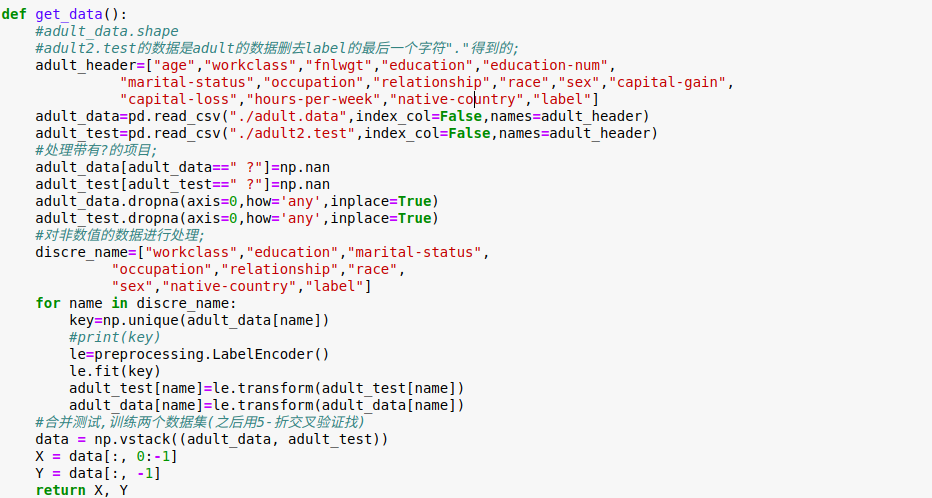
\includegraphics[scale=0.49]{hw51.png}
	%\caption{数据提取部分代码}
\end{figure}
	代码提取部分主要是从adult.data以及adult2.test里面获得数据,并且通过dropna将有" ?"的数据去掉;最后返回组合好了的X,Y以供后面的函数调用进行5折交叉验证;
\item[1.2.2]Random forest类:
\begin{itemize}

\item 参数:

n\_estimators=0 \# 树的数量

max\_features=0 \#每棵树的选用数据集的最大特征数

min\_samples\_split=0 \#每棵树最小分割数

min\_gain=0 \#每一颗树到min\_gain之后就停止

max\_depth=0 \#每一颗树的最大层数

trees=[~] \#森林

trees\_feature=[~] \#用来记录每一个树用了哪些特征
\item 函数:

\item def \_\_init\_\_ 是常规的初始化操作;
\item def get\_bootstrap\_data(self,X,Y):通过有放回的随机化,随机出一个大小和之前一样大的数据集,用于下面随机森林的训练;
\item def fit(self,X\_train,Y\_train):
\begin{figure}[!htbp]
	\centering
	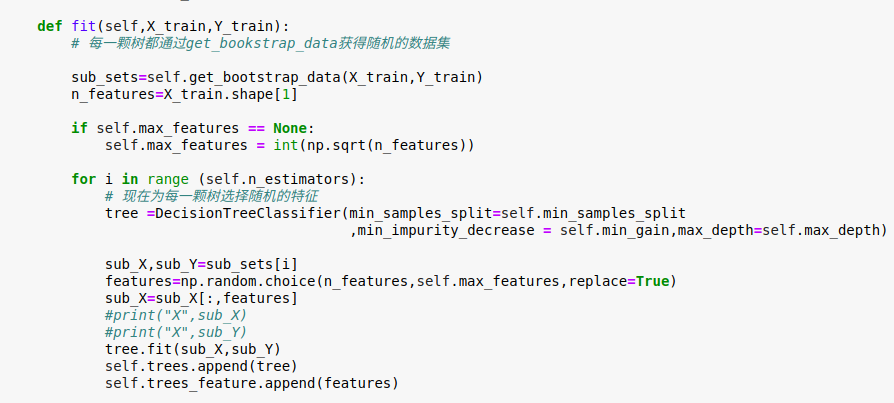
\includegraphics[scale=0.49]{randomfit.png}
	%\caption{数据提取部分代码}
\end{figure}
运用伪代码的算法如上图代码所示;
\item def predict(self,X):
我想了两个方案来通过上面的随机树来获得结果:

方案一是获得众数,用出现最多的(0/1)直接作为结果;

方案二是获得平均值,最后我选择的方案二,作为最后的答案输出;
\begin{figure}[!htbp]
	\centering
	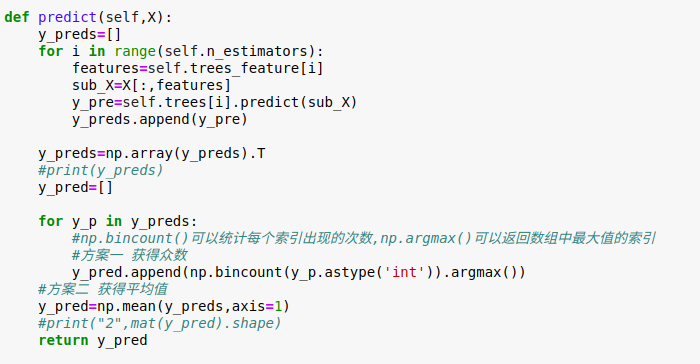
\includegraphics[scale=0.46]{randompredict.png}
	%\caption{数据提取部分代码}
\end{figure}

\newpage
\end{itemize}

\end{enumerate}
\item[2]对我adaboost部分的代码解释;
\begin{enumerate}
\item[2.1]数据提取部分和1.2.1用的是一样的函数;
\item[2.2]AdaBoost类:
\begin{itemize}
\item 参数:

T=500 \#用来确定训练的基分类器个数

weakClassArr=[~] \#用来存基分类器的alpha

weakalpha=[~]    \#用来存基分类器

max\_depth=0     \#用来确定树的最大depth

\item 函数:
\item 函数的实现基本和书上的伪代码一致,唯一有一些区别的是我在predict里面返回的是加权之后的小数,没有用sgn函数进行0/1化;
\end{itemize}
\end{enumerate}
\item[3] 关于交叉验证部分的代码:
\begin{figure}[!htbp]
	\centering
	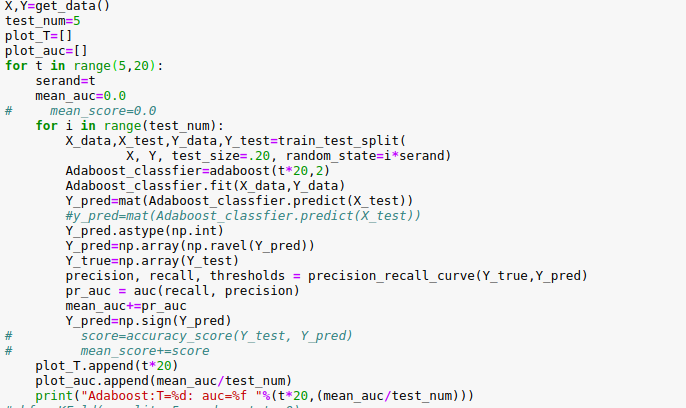
\includegraphics[scale=0.49]{auc.png}
	%\caption{数据提取部分代码}
\end{figure}

我手动设置了range的范围以及t乘以的系数,对于范围内的t我都将做test\_num次基于5折交叉验证的adaboost或者random forest的训练并且计算平均的auc;
基于这些平均的auc我也得到了相应的图像;
\item[4] 基学习器与AUC数据的关系,我根据数据做了相应的图像:
\begin{itemize}
	\item Randforest: 
	\begin{figure}[!htbp]
		\centering
		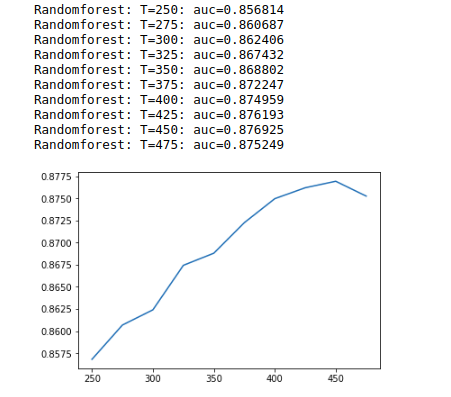
\includegraphics[scale=0.60]{randresult.png}
		%\caption{数据提取部分代码}
	\end{figure}
	\item AdaBoost:
	\begin{figure}[!htbp]
		\centering
		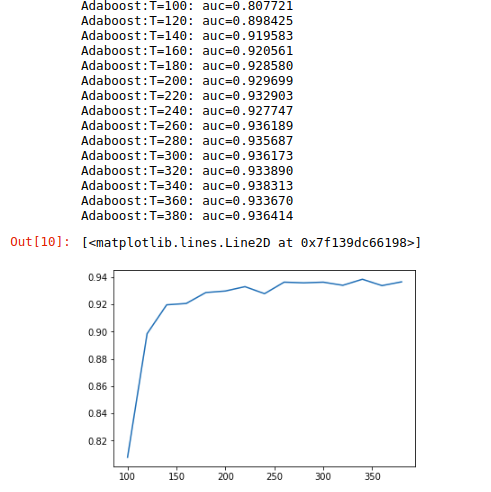
\includegraphics[scale=0.60]{adaboostresult3.png}
		%\caption{数据提取部分代码}
	\end{figure}
\end{itemize}
\item [5] 最后根据上面的分析,我选择 T=450 作为Randforest的参数,此时的AUC为0.876925;我选择T=380作为AdaBoost的参数,此时auc=0.936414
\item [6] 主要遭遇的bug是矩阵计算时候时候的shape问题,以及对python各种库函数的不熟悉,每一次都需要现场找,导致我花了一整天才完成不涵盖调参的工作;
\item [Hint] 现在我提交的py文件里面为了减少助教的审核时间用的是比较简单的参数,可能导致结果和上面不一样,以及请使用我转化过的adult2.test进行代码复现;我使用jupyter notebook写的代码,原来的代码在两个.ipynb文件里面,参数也是报告用的参数;
\end{enumerate}
\end{enumerate}
\end{solution}




%\begin{problem}[ML problem 5]

	%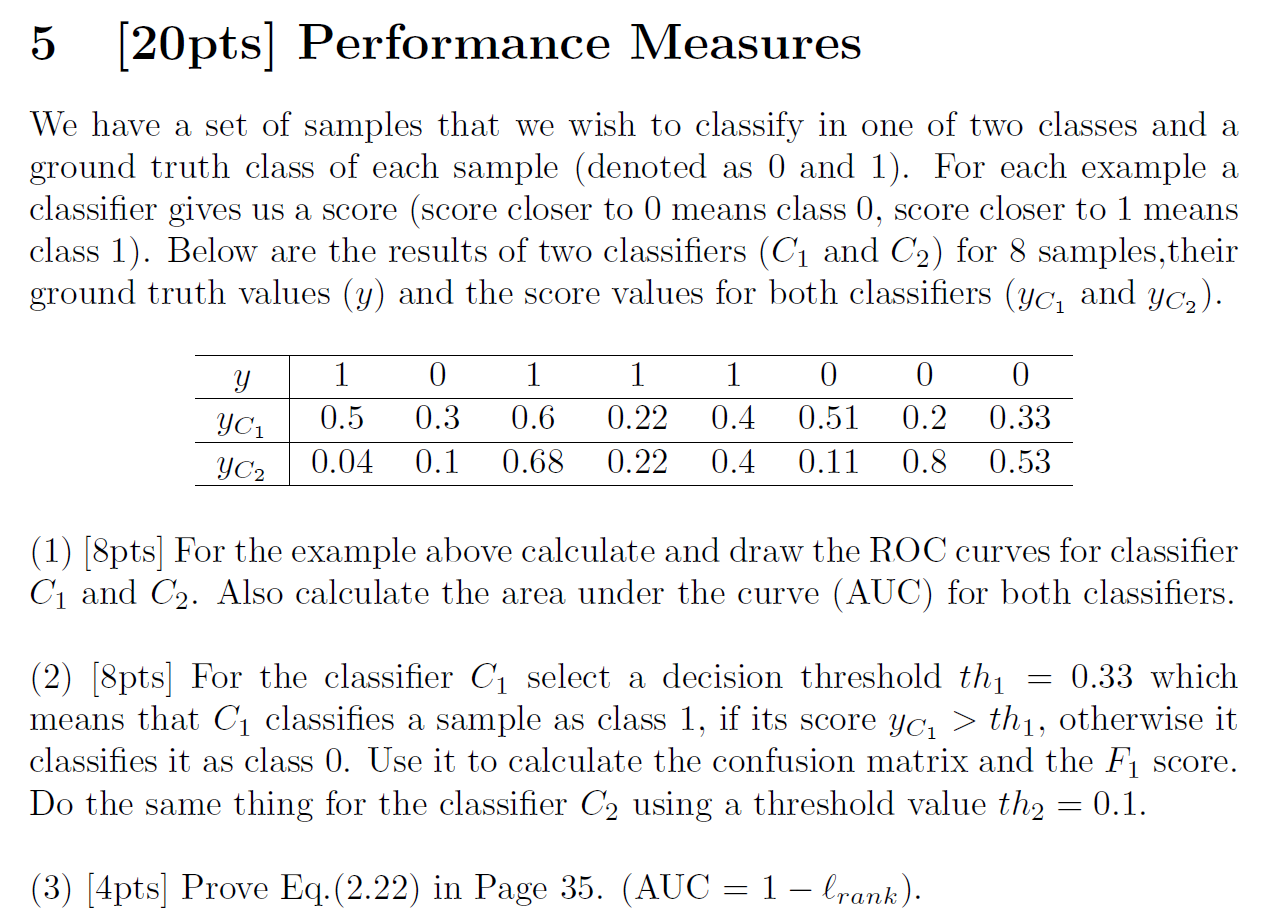
\includegraphics[scale=0.3]{5-p.png}

%\end{problem}
%\newpage
%\begin{solution}
   
%\end{solution}





%\begin{problem}[ML problem 6]
	
%\end{problem}
%\begin{solution}
    
%\end{solution}
%%%%%%%%%%%%%%%%%%%%%%%%%%%%%%%%%%%%%%%%%%%%%%%%%%%%%%%%%%%%%%%%
%                      Correction START!                       %
%%%%%%%%%%%%%%%%%%%%%%%%%%%%%%%%%%%%%%%%%%%%%%%%%%%%%%%%%%%%%%%%
%\begincorrection
%%%%%%%%%%%%%%%%%%%%
%\begin{problem}[]

%\end{problem}

%\begin{cause}
%
%\end{cause}

%\begin{revision}

%\end{revision}
%%%%%%%%%%%%%%%%%%%%
%\newpage
%%%%%%%%%%%%%%%%%%%%





%%%%%%%%%%%%%%%%%%%%%%%%%%%%%%%%%%%%%%%%%%%%%%%%%%%%%%%%%%%%%%%%
%                       Feedback START!                        %
%%%%%%%%%%%%%%%%%%%%%%%%%%%%%%%%%%%%%%%%%%%%%%%%%%%%%%%%%%%%%%%%
%\beginfb
%\begin{itemize}
%
%\end{itemize}





%%%%%%%%%%%%%%%%%%%%%%%%%%%%%%%%%%%%%%%%%%%%%%%%%%%%%%%%%%%%%%%%
%                        Homework END!                         %
%%%%%%%%%%%%%%%%%%%%%%%%%%%%%%%%%%%%%%%%%%%%%%%%%%%%%%%%%%%%%%%%
\end{document}
